%===============================================================================
% LaTeX sjabloon voor de bachelorproef toegepaste informatica aan HOGENT
% Meer info op https://github.com/HoGentTIN/bachproef-latex-sjabloon
%===============================================================================

\documentclass{bachproef-tin}

\usepackage{hogent-thesis-titlepage} % Titelpagina conform aan HOGENT huisstijl

%%---------- Documenteigenschappen ---------------------------------------------

% De titel van het rapport/bachelorproef
\title{Opschalen van een autodeelsysteem: optimalisatie van het reservatiealgoritme}

% Je eigen naam
\author{Tim Alenus}

% De naam van je promotor (lector van de opleiding)
\promotor{Wim Goedertier}

% De naam van je co-promotor. Als je promotor ook je opdrachtgever is en je
% dus ook inhoudelijk begeleidt (en enkel dan!), mag je dit leeg laten.
\copromotor{Rik Bellens}

% Indien je bachelorproef in opdracht van/in samenwerking met een bedrijf of
% externe organisatie geschreven is, geef je hier de naam. Zoniet laat je dit
% zoals het is.
\instelling{Partago}

% Academiejaar
\academiejaar{2018-2019}

% Examenperiode
%  - 1e semester = 1e examenperiode => 1
%  - 2e semester = 2e examenperiode => 2
%  - tweede zit  = 3e examenperiode => 3
\examenperiode{3}

%===============================================================================
% Inhoud document
%===============================================================================

\begin{document}

%---------- Taalselectie -------------------------------------------------------
% Als je je bachelorproef in het Engels schrijft, haal dan onderstaande regel
% uit commentaar. Let op: de tekst op de voorkaft blijft in het Nederlands, en
% dat is ook de bedoeling!

%\selectlanguage{english}

%---------- Titelblad ----------------------------------------------------------
\inserttitlepage

%---------- Samenvatting, voorwoord --------------------------------------------
\usechapterimagefalse
%%=============================================================================
%% Voorwoord
%%=============================================================================

\chapter*{\IfLanguageName{dutch}{Woord vooraf}{Preface}}
\label{ch:voorwoord}

%% TODO:
%% Het voorwoord is het enige deel van de bachelorproef waar je vanuit je
%% eigen standpunt (``ik-vorm'') mag schrijven. Je kan hier bv. motiveren
%% waarom jij het onderwerp wil bespreken.
%% Vergeet ook niet te bedanken wie je geholpen/gesteund/... heeft


%%=============================================================================
%% Samenvatting
%%=============================================================================

% TODO: De "abstract" of samenvatting is een kernachtige (~ 1 blz. voor een
% thesis) synthese van het document.
%
% Deze aspecten moeten zeker aan bod komen:
% - Context: waarom is dit werk belangrijk?
% - Nood: waarom moest dit onderzocht worden?
% - Taak: wat heb je precies gedaan?
% - Object: wat staat in dit document geschreven?
% - Resultaat: wat was het resultaat?
% - Conclusie: wat is/zijn de belangrijkste conclusie(s)?
% - Perspectief: blijven er nog vragen open die in de toekomst nog kunnen
%    onderzocht worden? Wat is een mogelijk vervolg voor jouw onderzoek?
%
% LET OP! Een samenvatting is GEEN voorwoord!

%%---------- Nederlandse samenvatting -----------------------------------------
%
% TODO: Als je je bachelorproef in het Engels schrijft, moet je eerst een
% Nederlandse samenvatting invoegen. Haal daarvoor onderstaande code uit
% commentaar.
% Wie zijn bachelorproef in het Nederlands schrijft, kan dit negeren, de inhoud
% wordt niet in het document ingevoegd.

\IfLanguageName{english}{%
\selectlanguage{dutch}
\chapter*{Samenvatting}
\selectlanguage{english}
}{}

%%---------- Samenvatting -----------------------------------------------------
% De samenvatting in de hoofdtaal van het document

\chapter*{\IfLanguageName{dutch}{Samenvatting}{Abstract}}
Partago is een coöperatie die elektrisch autodelen aanbiedt aan haar leden en in volle groei is. Om elektrisch autodelen zorgeloos te maken ontwikkelde Partago een eigen autodeelplatform. Als de gebruikersaantallen van Partago blijven groeien zal er vroeg of laat een opschaling nodig zijn van het huidige reserveringssysteem. Dit onderzoek onderzoekt één van de mogelijke optimalisaties: de gebruiker niet zelf een auto laten kiezen tijdens het reserveren, maar een auto laten toewijzen door een algoritme zodat de beschikbare auto's optimaal worden ingevuld. Zulk toewijzingsprobleem kan geformuleerd worden aan de hand van een Constraint Satisfaction Problem, afgekort tot CSP. Op basis van een dataset van historische reservaties werden, met een zelf gecodeerde simulatietool, simulaties uitgevoerd voor een periode van 4 weken telkens met een verschillend aantal reservaties en een verschillend aantal beschikbare auto's. Voor elke simulatie werd de toewijzing van auto's aan reservaties éénmaal willekeurig gedaan en éénmaal aan de hand van de oplossing van het corresponderende Constraint Satisfaction Problem. Voor zowel de willekeurige toewijzing als voor de toewijzing met behulp van een CSP werd het service level, gedefinieerd als het percentage van reservaties dat kan doorgaan, en de totale actieve tijd per auto berekend. Uit de resultaten van de simulaties kan afgeleid worden dat er maar kleine winstmarges te boeken zijn voor het service level en de actieve tijd per auto door gebruik te maken van een CSP in vergelijking met de eenvoudige toewijzing. Naarmate het systeem drukker en complexer wordt, meer reservaties en meer auto's, lijken de winstmarges te groeien. Echter door het gebruik van een niet-performant algoritme om het CSP op te lossen was dit onderzoek gelimiteerd om de complexiteit van de gesimuleerde systemen op te drijven. Een vervolg op dit onderzoek zou een meer geavanceerd algoritme kunnen gebruiken om het CSP op te lossen.


%---------- Inhoudstafel -------------------------------------------------------
\pagestyle{empty} % Geen hoofding
\tableofcontents  % Voeg de inhoudstafel toe
\cleardoublepage  % Zorg dat volgende hoofstuk op een oneven pagina begint
\pagestyle{fancy} % Zet hoofding opnieuw aan

%---------- Lijst figuren, afkortingen, ... ------------------------------------

% Indien gewenst kan je hier een lijst van figuren/tabellen opgeven. Geef in
% dat geval je figuren/tabellen altijd een korte beschrijving:
%
%  \caption[korte beschrijving]{uitgebreide beschrijving}
%
% De korte beschrijving wordt gebruikt voor deze lijst, de uitgebreide staat bij
% de figuur of tabel zelf.

\listoffigures
\listoftables

% Als je een lijst van afkortingen of termen wil toevoegen, dan hoort die
% hier thuis. Gebruik bijvoorbeeld de ``glossaries'' package.
% https://www.overleaf.com/learn/latex/Glossaries

%---------- Kern ---------------------------------------------------------------

% De eerste hoofdstukken van een bachelorproef zijn meestal een inleiding op
% het onderwerp, literatuurstudie en verantwoording methodologie.
% Aarzel niet om een meer beschrijvende titel aan deze hoofstukken te geven of
% om bijvoorbeeld de inleiding en/of stand van zaken over meerdere hoofdstukken
% te verspreiden!

%%=============================================================================
%% Inleiding
%%=============================================================================

\chapter{\IfLanguageName{dutch}{Inleiding}{Introduction}}
\label{ch:inleiding}

Partago is een start-up en een coöperatie die elektrische auto's beschikbaar stelt aan haar coöperanten om te delen. Om dit mogelijk te maken heeft Partago een eigen software platform ontwikkeld: het Partago Platform. Deze software wil voldoen aan de specifieke noden die ontstaan wanneer een groep van gebruikers onderling elektrische auto's willen delen. Deze groep van burgers kunnen de coöperanten zelf zijn, maar even goed een lokale overheid of een bedrijf dat elektrische auto's wil delen onder haar werknemers. Het Partago platform bestaat uit een applicatie voor de smartphone en een managementtool om de operationele processen die gepaard gaan met het delen van een elektrische vloot te ondersteunen. Een RESTful webservice zorgt voor een laag tussen de app en de database en handelt onder andere reserveringen af.

\section{\IfLanguageName{dutch}{Probleemstelling}{Problem Statement}}
\label{sec:probleemstelling}
Partago-auto's leven in zones. Het gebruik van een auto start en eindigt in de thuiszone van de wagen. Een voorbeeld van een zone is "Brugse Poort". Een auto met als thuiszone de Brugse Poort zal dus, wanneer niet in gebruik, geparkeerd zijn in deze wijk. Meerdere auto's kunnen dezelfde zone als thuisbasis hebben. Naarmate de vloot groeit binnen één stad is het misschien zelfs opportuun om de gehele stad als één zone te aanzien. Dit is nu nog niet het geval. Vanaf een gebruiker het gebruik start is hij vrij waarheen hij reist, maar het gebruik kan pas terug worden afgesloten wanneer de auto zich terug in de thuiszone bevindt. Momenteel maakt een gebruiker een reservatie voor een specifieke auto of kiest hij voor spontaan gebruik van een specifieke auto. Hierdoor wordt er echter niet optimaal gebruik gemaakt van de verschillende auto's die beschikbaar zijn binnen de zone. Een voorbeeld: Karel, Joachim en Clara willen allen gebruik maken van een auto in de zone Brugse Poort. De Brugse Poort is de thuislocatie van twee auto's: auto1 en auto2. Karel maakt een reservatie voor auto1 van 10h tot 12h. Joachim maakt een reservatie voor auto2 van 14h-17h. Clara wil ook gebruik maken van een Partago-auto. Zij zou de auto nodig hebben van 11h tot 16h. Er is echter geen enkele auto beschikbaar voor die tijdsspanne. Moesten echter Karel en Joachim beide gebruik maken van auto1 zou Clara perfect nog gebruik kunnen maken van auto2. Het systeem dwingt dit echter op geen enkele manier af. Een alternatieve manier om het reserveringssysteem op te stellen zou zijn dat de gebruikers geen specifieke auto reserveren, maar een zone. Zo zou het systeem voor de zone reservaties ontvangen van Karel voor 10h tot 12h, van Joachim voor 14h tot 17h en van Clara voor 11h tot 16h. Het systeem zou dan zelf een toewijzing kunnen doen om zoveel mogelijk gebruikers tevreden te stellen.

\section{\IfLanguageName{dutch}{Onderzoeksvraag}{Research question}}
\label{sec:onderzoeksvraag}

Met het onderzoek beschreven in deze bachelorproef willen we een antwoord vinden op de vraag of het service level en de gebruiksduur van de auto's van Partago stijgt wanneer de gebruikers geen specifieke auto's reserveren, maar enkel een zone. Nadien wordt dan door het systeem een toewijzing gedaan wie welke fysieke auto toegewezen krijgt. Deze onderzoeksvraag vormt de kern van het onderzoek. We definiëren het service level als het percentage van aangevraagde ritten dat daadwerkelijk ook kan doorgaan omdat er minstens nog één auto vrij is. Tevens zullen we enkele bijkomende, secundaire onderzoeksvragen willen beantwoorden. Hoe kunnen we het systeem de toewijzing laten doen en heeft deze wijziging van het reservatiemechanisme implicaties op het ontwerp van de databank en de rest van het systeem.

\section{\IfLanguageName{dutch}{Onderzoeksdoelstelling}{Research objective}}
\label{sec:onderzoeksdoelstelling}

Voor het onderzoek beogen we een simulatietool te ontwikkelen om de verschillende situaties tussen reserveren per auto en het reserveren per zone te simuleren. Uit deze simulaties zullen we kunnen trekken welke aanpak bij welke parameters de voorkeur heeft. Met de simulatietool moet het mogelijk zijn het aantal gebruikers en het aantal auto's in de zone te laten variëren. Voor elke specifieke combinatie van parameters beoogt de simulatietool een toewijzing te doen van auto's aan reservaties. Bij elke toewijzing hoort een service level berekent te worden alsook de tijd dat de auto's actief waren. Door de verschillende parameters te laten variëren kan er hopelijk een conclusie getrokken worden bij welk aantal gebruikers en bij welke grootte van de vloot het voor Partago opportuun wordt om het reserveringsmechanisme aan te passen naar een meer geavanceerde en geoptimaliseerde versie.

\section{\IfLanguageName{dutch}{Opzet van deze bachelorproef}{Structure of this bachelor thesis}}
\label{sec:opzet-bachelorproef}

% Het is gebruikelijk aan het einde van de inleiding een overzicht te
% geven van de opbouw van de rest van de tekst. Deze sectie bevat al een aanzet
% die je kan aanvullen/aanpassen in functie van je eigen tekst.

De rest van deze bachelorproef is als volgt opgebouwd:

In Hoofdstuk~\ref{ch:stand-van-zaken} wordt een overzicht gegeven van de stand van zaken binnen het onderzoeksdomein. We bespreken eerder gedaan onderzoek op de vloot van Partago. We bekijken hoe we het systeem zo correct mogelijk kunnen modelleren en bouwen een solide theoretische basis op om de lezer van deze bachelorproef vertrouwd te maken met de materie.

In Hoofdstuk~\ref{ch:methodologie} wordt de methodologie toegelicht. We beschrijven hoe we te werk zijn gegaan om een antwoord te kunnen formuleren op de onderzoeksvragen en duiden de gebruikte onderzoekstechnieken.

In Hoofdstuk ~\ref{ch:resultaten-simulaties} voeren we verschillende simulaties uit met de ontwikkelde simulatietool. We laten het aantal reservaties en het aantal auto's variëren zowel bij willekeurig toewijzen van een auto als bij gebruik van het toewijzingsalgoritme.

In Hoofdstuk~\ref{ch:conclusie}, tenslotte, wordt de conclusie gegeven en een antwoord geformuleerd op de verschillende onderzoeksvragen. Aansluitend wordt ook een aanzet gegeven voor toekomstig onderzoek binnen dit domein.
\chapter{\IfLanguageName{dutch}{Stand van zaken}{State of the art}}
\label{ch:stand-van-zaken}

% Tip: Begin elk hoofdstuk met een paragraaf inleiding die beschrijft hoe
% dit hoofdstuk past binnen het geheel van de bachelorproef. Geef in het
% bijzonder aan wat de link is met het vorige en volgende hoofdstuk.

% Pas na deze inleidende paragraaf komt de eerste sectiehoofding.

\section{Wat is autodelen?}
Autodelen bestaat ondertussen zo'n 15-tal jaar in België \autocite{ing}, autodelen is echter geen recent fenomeen. Volgens \textcite{millardball} vinden we de eerste pogingen van een vastgestelde autodeelorganisatie terug in de jaren '40 in een coöperatief samenwoon-project in het Zwitserse Zürich. Het meeste onderzoek gedaan rond autodelen geeft echter geen formele definitie van wat autodelen nu exact is \autocite{millardball}. In dit onderzoek zullen we autodelen definiëren als ``de toegang, via een abonnement of bundel, tot een vloot auto's via het zelfbedieningsprincipe, beschikbaar voor korte periodes en korte afstanden, waarvoor de gebruiker (particulier of bedrijf) een toeslag per uur en/of per afgelegde kilometer betaald`` \autocite{ing}.

\section{Wachtrijtheorie}
Een mogelijke aanpak voor het modelleren van een reservatiesysteem zoals dat van Partago is met behulp van wachtrijtheorie. In de masterthesis Dimensionering van een autodeelsysteem aan de hand van wachtrijtheorie beschrijft \textcite{van-buggenhout} hoe een reservatiesysteem gemodeleerd kan worden aan de hand van wachtrijtheorie. Verder in dit onderzoek zal er geen gebruik gemaakt worden van wachtrijtheorie, het is echter belangrijk om deze mogelijke aanpak toch kort toe te lichten. In wat volgt vatten we kort samen hoe het systeem gemodelleerd kan worden aan de hand van wachtrijtheorie.

\subsection{Wat is wachtrij theorie}
Een wachtrijmodel beschrijft een systeem waarbij klanten arriveren bij het systeem op verschillende tijdstippen, wachten tot het hun beurt is om door het systeem geserveerd te worden en tenslotte het systeem terug verlaten. Het doel van wachtrijtheorie is een balans te vinden tussen de service naar klanten toe en het aantal servers. Meer servers betekend doorgaans hogere kosten. \textcite{van-buggenhout}. Naar Partago toe kunnen we de servers vertalen naar auto's. Hoe meer auto's hoe meer klanten Partago kan serveren, maar hoe meer auto's hoe hoger de operationele kosten. 

Om het systeem correct te modelleren aan de hand van wachtrijtheorie moeten we de volgende parameters kennen:
\begin{itemize}
	\item de grootte van de populatie van klanten
	\item het type aankomstproces 
	\item de capaciteit van de wachtrij
	\item het type serviceproces
	\item het aantal beschikbare servers
\end{itemize}

\subsection{Grootte van de klantenpopulatie}
Er wordt een onderscheidt gemaakt tussen eindige en oneindige klantenpopulaties. Om gebruik te kunnen maken van de Partagoauto's moet je coöperant zijn van Partago. Het systeem kent dus ten alle tijden een bovengrens voor de klantenpopulatie en is dus eindig, namelijk het aantal coöperanten.

\subsection{Aankomstproces}
Elke Partago-coöperant heeft zijn eigen mobiliteitsbehoeften. Er wordt vanuit gegaan dat deze mobiliteitsbehoeften willekeurig en geheugenloos zijn. Geheugenloos wil zeggen dat het tijdstip van het huidige gebruik van het systeem onafhankelijk is van het vorige gebruik. Als er tijdens een bepaalde periode  $P_{1}$ een aantal reserveringen waren dan heeft dit geen invloed op hoeveel er zullen zijn in een andere periode $P_{2}$. Er wordt gesproken van willekeur omdat de reservaties niet uniform aan het systeem toekomen. Als er geweten is dat er tijdens een bepaalde periode gemiddeld 6 reservaties per uur zijn wil dit niet zeggen dat deze 6 reservaties mooi om de tien minuten plaatsvinden. Om met deze willekeur overweg te kunnen zal het aankomstproces gemodelleerd worden door middel van een statistische verdeling. Een discreet aankomstproces dat geheugenloos en willekeurig is kan gemodelleerd worden aan de hand van een Poisson-proces. Een Poisson-proces is een proces waarbij het aantal aankomsten verdeeld is volgens een Poisson-distributie terwijl de tijd tussen 2 aankomsten exponentieël verdeeld is. Een Poisson-proces wordt gekarakteriseerd volgens de aankomstsnelheid $\Lambda$ \autocite{liu}. Een belangrijke kanttekening die  hierbij gemaakt moeten worden is dat deze parameter voor het systeem van Partago wel afhankelijk is van de tijd. Zo is het weekend bijvoorbeeld drukker. Tijdens het weekend zal er dus een hogere aankomstsnelheid gemeten kunnen worden. \autocite{van-buggenhout}

\subsection{Capaciteit van de wachtrij}
Wanneer een gebruiker niet geserveerd kan worden door Partago zal deze gebruiker zijn mobiliteitsbehoeften elders moeten vervullen. Er staan dus nooit gebruikers in de wachtrij. De grootte van de wachtrij is met andere woorden nul.

\subsection{Serviceproces}
Het Partago systeem serveert een gebruiker wanneer deze gebruiker gebruik maakt van de gereserveerde auto. De service tijd wordt gedefinieerd als de tijd dat een gebruiker gebruik maakt van het systeem. De service tijden van alle gebruikers en servers zijn onafhankelijk van elkaar en worden veronderstelt exponentieel verdeelt te zijn en dus te modelleren zijn als poissonprocessen. De kans dat een gebruiker zijn gebruik van de auto beëindigt is onafhankelijk van de tijd reeds gebruik gemaakt van de auto.

\subsection{Beschikbare servers}
Het systeem bestaat uit een vast aantal auto's. Het systeem weet ook ten alle tijden welke auto's beschikbaar zijn en welke niet.

\subsection{Conclusie}
Aan de hand van wachtrijtheorie kon \textcite{van-buggenhout} een model creëren voor het Partago systeem. Dit model werd in een java-applicatie gegoten. Met behulp van deze applicatie werd de optimale vlootgrootte berekent voor de verschillende zones waar Partago actief was op het moment van schrijven van van Buggenhout's onderzoek. Als waarde voor de aankomstsnelheid voor het Poisson aankomstproces werd de aankomstsnelheid van de historisch drukste ochtend van die bepaalde zone gekozen. Uit het onderzoek werd geconcludeerd dat om het service level op 95\% te krijgen er in alle zones één auto moet bijkomen. Dit heeft echter een zeer negatief effect op de bezettingsgraad van de vloot. De impact van de verschillende parameters kan als volgt worden samengevat. 
\begin{center}
	\begin{tabular}{ | l | l | p{3cm} |}
		\hline
		Parameter & Relatie tot service level (QoS) & Impact op service level \\ \hline
		Aankomstsnelheid $A_{p}$ & $A_{p}$ $\uparrow$ = $QoS$ $\downarrow$ & hoog \\ \hline
		Aantal auto's $m$ & $m$ $\uparrow$ = $QoS$ $\uparrow$ & hoog \\ \hline
		Gemiddelde gebruikstijd $MST$ & $MST$ $\uparrow$ = $QoS$ $\downarrow$ & hoog \\ \hline
		Aantal gebruikers $S$ & $S$ $\uparrow$ = $QoS$ $\downarrow$ & laag \\ \hline
	\end{tabular}
\end{center} 
In deze bachelorproef zal echter geen gebruik gemaakt worden van wachtrijtheorie. Het onderzoek van \textcite{van-buggenhout} werd geschreven kort na de oprichting van Partago en het systeem bevond zich dus nog in een zeer vroeg stadium. Voor dit onderzoek wordt gebruik gemaakt van een grote hoeveelheid historische reservaties als input voor het uitvoeren van de simulaties. In het hoofdstuk ~\ref{ch:methodologie} wordt verder uitgelegd hoe te werk is gegaan.

\section{Constraint Satisfaction Problem}

De doelstelling van dit onderzoek is een antwoord formuleren op de vraag of het invoeren van een toewijzingsalgoritme voor de reservaties tot een hogere service level zal leiden. Een toewijzingsprobleem kan herleid worden tot een Constraint Satisfaction Problem.

\subsection{Definitie}
Het toewijzen welke reservatie zal doorgaan met welke auto kan herleidt worden tot een Constraint Satisfaction Problem in het kort een CSP. Een CSP is gedefinieerd door een set \textbf{variabelen} $X_{1}$, $X_{2},...,X_{n}$ en een set \textbf{constraints} $C_{1}, C_{2},...C_{m}$. Elke variabele $X_{i}$ heeft een niet leeg \textbf{domein} $D_{i}$ van mogelijke waarden. Elke constraint $C_{i}$ heeft betrekking tot een subset van de variabelen en specificeert de mogelijke combinaties van waarden voor deze subset. Een toestand van het probleem is gedefinieerd als een \textbf{toewijzing} van waarden aan sommige van de variabelen $X_{i} =  v_{i}, X_{j} = v_{j}$... Een toewijzing dat geen enkele van de constraints schendt is een \textbf{consistente} of legale toewijzing. Een volledige toewijzing of \textbf{oplossing} van het CSP is een toewijzing waarin alle variabelen vernoemd worden en aan alle constraints is voldaan. Soms moet een oplossing van een CSP er ook naar streven een strafscore te minimaliseren \autocite{norvig}.

\subsection{Oplossen van een CSP}
Het oplossen van een CSP is een complexe aangelegenheid. Voor het oplossen van zulke problemen worden steeds krachtigere algoritmes ontwikkeld. Een standaard algoritme kan een diepte-eerst backtracking search zijn \autocite{norvig}. Deze aanpak is relatief eenvoudig in implementatie en is ook het soort algoritme dat gebruikt wordt in de softwarebibliotheek die later in dit onderzoek gebruikt wordt.
\paragraph{Diepte-eerst zoeken}
Diepte eerst zoeken is een blinde zoekmethode. Dit wil zeggen dat ze enkel gebruik kunnen maken van de informatie verschaft in de definitie van het probleem \autocite{lievens}. Bij diepte-eerst zoeken wordt een open lijst gebruikt. Deze open lijst bestaat uit mogelijke partiële oplossingen (plannen) die nog verder geëxpandeerd moeten worden. Bij diepte-eerst zoeken wordt deze open-lijst bijgehouden in een LIFO-structuur (Last In First Out). Dit zorgt ervoor dat men steeds zo snel mogelijk zo diep mogelijk afdaalt in de zoekboom. \begin{figure}[h]
	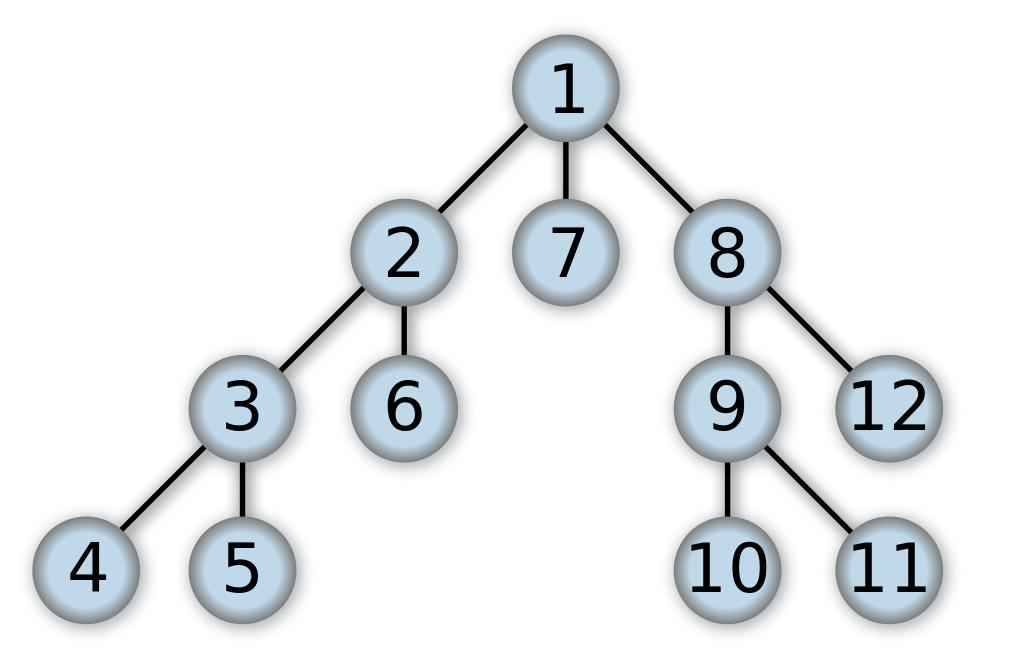
\includegraphics[width=\textwidth]{diepte-eerst.png}
	\caption{visuele voorstelling de zoekboom bij diepte-eerst zoeken}
\end{figure}
Wanneer diepte eerst een oplossing vindt is deze niet gegarandeerd een optimale oplossing. De oplossing ontdekt door diepte eerst is immers steeds de ``meest linkse`` doeltop. Wanneer het aantal verschillende mogelijke toestanden eindig is en de doeltop bevindt zich helemaal rechts onderaan de zoekboom dan worden alle toppen van de boom doorlopen door het zoekalgoritme. Diepte-eerst heeft dus in het slechtste geval een exponentiële tijdscomplexiteit van $\Theta(b_{m})$ \autocite{lievens}. $b$ is het aantal broers van een knoop in de boom (dus het aantal mogelijke domeinwaarden) en $m$ het aantal niveau's in de boom (dus het aantal variabelen).

\paragraph{Backtracking search}
Backtracking search is een algoritme dat diepte eerst te werk gaat om op zoek te gaan naar een oplossing van een CSP probleem. Het kiest waarden voor één variabele tegelijk en traceert terug in de boom wanneer er geen domeinwaarden meer mogelijk zijn om toe te wijzen aan een variabele. Eén voor een worden niet geässigneerde variabelen geprobeerd, voor elke variabele wordt dan elke domeinwaarde uitgeprobeerd \autocite{norvig}. De volgorde dat de variabelen doorlopen worden en de volgorde dat de domeinwaarden geprobeerd worden heeft een grote invloed op de uiteindelijke oplossing die het algoritme zal ``tegenkomen``. Door het wijzigen van deze volgordes op basis heuristieken  die extra informatie aan het algoritme verschaffen zal het algoritme beter presteren. Een voorbeeld van zo'n heuristiek is om de uit te proberen domeinwaarden te sorteren op de minst beperkende domeinwaarde. Met andere woorden de eerste domeinwaarde die wordt uitgeprobeerd is degene die het minst voorkomst in de constraints voor deze variabele. Jammer genoeg maakt de softwarebibliotheek die verder in dit onderzoek gebruikt wordt nog geen gebruik van deze heuristieken.


%%=============================================================================
%% Methodologie
%%=============================================================================

\chapter{\IfLanguageName{dutch}{Methodologie}{Methodology}}
\label{ch:methodologie}

\section{Type onderzoek}
Het onderzoek beschreven in deze tekst is een \textbf{kwantitatief} onderzoek. Voor combinaties van het aantal auto's en het aantal reservaties zullen het service level, de totale gebruiksduur van de auto's en de tijdsduur van de reservaties die niet konden doorgaan vergeleken worden. Vanuit een bedrijfsstandpunt is het interessant om het service level en de gebruiksduur van de auto's maximaliseren voor een gegeven grootte van de vloot. Voor dit onderzoek wordt geopteerd voor een aanpak die zo dicht mogelijk aansluit bij de realiteit binnen het bestek van het onderzoek. In plaats van de meer theoretische en wiskundige aanpak met wachtrijtheorie beschreven in de stand van zaken worden er in dit onderzoek simulaties uitgevoerd uit met een zelf-ontwikkelde simulatietool. De programmeercode van deze simulatietool is als bijlage opgenomen. Deze simulaties simuleren reëel reservatiegedrag van de Partago gemeenschap en zijn gebaseerd op historische reservaties van Partago. Verder in dit hoofdstuk wordt exact beschreven hoe deze simulaties zijn opgebouwd en welke stappen binnen elke simulatie uitgevoerd worden om tot numerieke waarden voor het service level en de gebruiksduur van de auto's te komen. 

\section{Opzet van een simulatie}
\subsection{Doel}
Tijdens de simulatie wordt er een getracht tweemaal een toewijzing te doen van de beschikbare auto's aan de reservaties in de simulatie. Eenmaal zal deze toewijzing gebeuren op een eenvoudige manier (zie verder) en eenmaal zal deze toewijzing gebeuren door het oplossen van het corresponderende Constraint Satisfaction Problem (zie verder en stand van zaken). Voor beide toewijzingen wordt dan het service level, de tijd dat de auto's actief waren en de tijd van reservaties die niet konden doorgaan omdat er geen auto beschikbaar was berekend. Elke karakteriserende simulatie wordt meermaals uitgevoerd om genoeg datapunten voor de grootheden te genereren. Hierdoor kan per set van karakteristieke parameters een gemiddelde en standaard afwijking berekent worden. 

\subsection{Karakteristieken}
Eén enkele simulatie wordt gekarakteriseerd door waarden van de volgende grootheden:
\begin{itemize}
	\item \textbf{Aantal reservaties in de simulatie:}
	Het aantal reservaties is een maat voor de drukte op het systeem. Het aantal gebruikers van het systeem zou hier geen goede maat voor zijn, weinig gebruikers kunnen immers ook relatief veel reservaties maken. Veel reservaties betekent een grote drukte op het systeem, weinig reservaties betekent een kleine drukte. Uiteraard kunnen overlappende reservaties niet van dezelfde persoon afkomstig zijn. De reservaties gebruikt in de simulatie zijn bestaande historische reservaties van Partago.
	\item \textbf{Aantal auto's:}
	Tijdens de simulatie zullen er toewijzingen gebeuren van de auto's aan de reservaties. Meer auto's beschikbaar in de fictieve zone zal het service level onmiddellijk doen toenemen. Voor eenzelfde aantal reservaties zullen meer reservaties kunnen doorgaan als er meer auto's beschikbaar zijn. 
	\item \textbf{Aantal weken:}
	Elke simulatie stelt een fictieve reserveringsperiode voor van een aantal weken. Tijdens dit onderzoek wordt deze parameter vastgehouden op \textbf{2 weken}. Tijdens elke simulatie zullen we dus een periode van 2 weken simuleren. 
\end{itemize} 

\subsection{Stappen binnen een simulatie}
Binnen één enkele simulatie worden de volgende stappen ondernomen
\begin{enumerate}
	\item Definiëren van de karakteriserende parameters
	\item Historische Partago reservaties ophalen
	\item Een dataset van reservaties genereren op basis van de historische gegevens voor de gedefinieerde periode
	\item Een eenvoudige toewijzing doen van auto's op de reservaties uit de dataset
	\item Een toewijzing doen van auto's op de reservaties uit de dataset met behulp van een CSP oplosalgoritme 
	
\end{enumerate}
Op elk van deze stappen wordt dieper ingegaan in de komende secties van dit hoofdstuk. 

\section{Definiëren van de karakteriserende parameters}
\subsection{Aantal reservaties}
\subsection{Aantal auto's}
\subsection{Aantal weken}
Zoals eerder vermeld zal deze parameter vastgehouden worden op 2 weken. Deze keuze is arbitrair. De simulaties over een langere periode laten lopen zou de rekentijd aanzienlijk verhogen en weinig meerwaarde bieden. Zoals eerder vermeld wordt een simulatie met een set van parameters meermaals uitgevoerd zodat de resultaten uitgemiddeld worden. 

\section{Partago reservaties ophalen}
De dataset van reservaties die gegenereerd wordt is gebaseerd op bestaande reservaties uit het verleden gedaan op het systeem van Partago. Dit geeft als voordeel dat de dataset een reëel karakter zal vertonen en dus dicht aansluit op werkelijk reserveringsgedrag. Voor dit onderzoek worden historische gegevens van Partago van 1 januari 2019 tot en met 30 juni 2019 gebruikt. Voor filtering zijn dit 7661 reservaties die gebruikt kunnen worden om datasets uit te generen. Dit aantal wordt wel nog opgekuist vooraleer de dataset gegenereerd wordt: reservaties niet uitgevoerd door Partago-coöperanten (bijvoorbeeld door het onderhoudsteam), reservaties korter dan 5 minuten, reservaties langer dan 24uur en geannuleerde reservaties worden verwijderd.

\section{Dataset van reservaties genereren}
Uit de gefilterde lijst van Partago reservaties zal een dataset van reservaties gegenereerd worden voor een periode van het gedefinieerde aantal weken. In dit onderzoek zal elke dataset dus bestaan uit reservaties voor 2 weken. De parameter "aantal reservaties" zal bepalen hoeveel reservaties zich in de dataset bevinden. Dit aantal wordt willekeurig geselecteerd uit de historische Partago reservaties en gemapt op een willekeurige week in de dataset (week1 of week2), maar met behoudt van de dag van de week. Reservatiegedrag op een dinsdag is mogelijks niet hetzelfde als reservatiegedrag op een zaterdag. Deze informatie mag dus niet verloren gaan tijdens het mappen. Aangezien de reservaties willekeurig geselecteerd worden zullen de reservaties per dag in een willekeurige volgorde staan. Dit is eveneens de volgorde waarmee de reservaties toekomen bij het systeem. Figuur3.1 is een visuele voorstelling van een eenvoudige dataset van 2 weken met 38 reservaties.
\begin{figure}[h]
	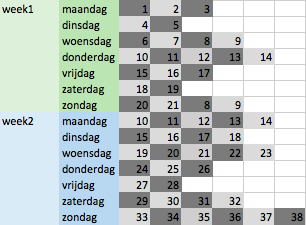
\includegraphics{dataset.png}
	\caption{visuele voorstelling van een dataset}
\end{figure}
\section{Eenvoudige toewijzing}
\section{Toewijzing met behulp van een CSP}







% Voeg hier je eigen hoofdstukken toe die de ``corpus'' van je bachelorproef
% vormen. De structuur en titels hangen af van je eigen onderzoek. Je kan bv.
% elke fase in je onderzoek in een apart hoofdstuk bespreken.
\chapter{\IfLanguageName{dutch}{Resultaten van de simulaties}{Results of the simulations}}
\label{ch:resultaten-simulaties}
In dit hoofdstuk worden de resultaten van de verschillende simulaties weergeven. De simulaties worden uitgevoerd met een zelf geschreven simulatietool waarvan de code zich in bijlage bevindt. Voor elke set van parameters in tabel \ref{tab:parameters} voeren we 30 maal een simulatie uit. De simulatietool slaat voor elke run van een simulatie het service level, de duur dat de auto's actief waren en de duur van reservaties die niet konden doorgaan omdat er geen auto beschikbaar was op in een bestand voor zowel de eenvoudige toewijzing als voor de CSP toewijzing. Deze bestanden worden geanalyseerd met behulp van een rekenblad.
In de volgende secties worden de resultaten van de simulaties weergeven met volgende symbolen:
\begin{itemize}
	\item $\mu_{ SL}$: het gemiddelde service level
	\item $\sigma^2$: standaardafwijking
	\item $\mu_{ t}$: gemiddelde actieve tijd
	\item $\mu_{\Delta_{ SL}}$: gemiddelde verbetering service level
	\item $\mu_{\Delta_{ t}}$: gemiddelde verbetering actieve tijd
\end{itemize}
Elke simulatie wordt 30 maal uitgevoerd. Een voorbeeld van de ruwe output data van een simulatie voor het service level wordt weergeven in figuur \ref{grafiek:ruwe-output-simulatie}. Een gelijkaardige grafiek kan opgesteld worden voor de actieve tijd van de auto's alsook van de tijd van de reservaties die niet konden doorgaan.
\begin{figure}[h]
	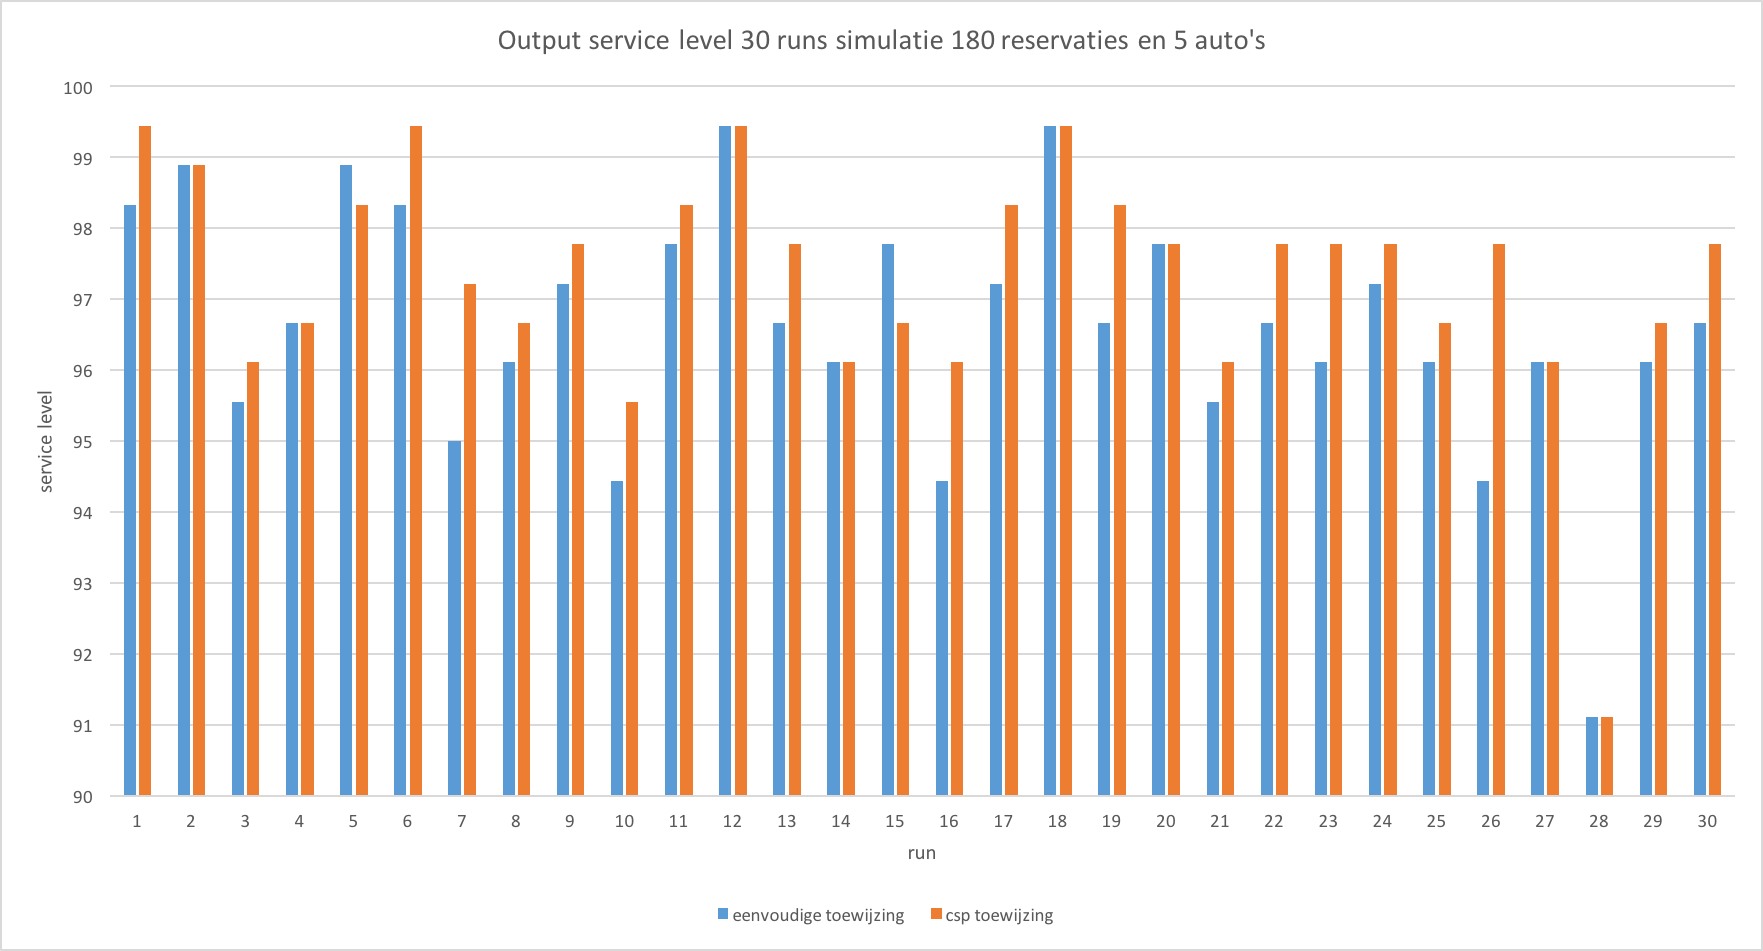
\includegraphics[width=\textwidth]{grafiek-ruwe-output-simulatie.png}
	\caption[Grafiek die de ruwe output data voor het service level van 30 runs van een simulatie weergeeft]{Grafiek die de ruwe output data voor het service level van 30 runs van een simulatie weergeeft}
	\label{grafiek:ruwe-output-simulatie}
\end{figure}

\section{Druktegraad: 9 reservaties/week/auto}
Er werden 2 sets van parameters samengesteld met een druktegraad van 9 reservaties per week per auto. 
De eerste simulatie bestaat uit 108 reservaties verdeeld over 4 weken voor 3 auto's, de tweede bestaat uit 180 reservaties verdeeld over 4 weken voor 5 auto's. 
De gemiddelde resultaten van de simulatie worden weergeven in tabel \ref{tab:resultaten9}
\begin{table}[h]
	\centering
	\begin{tabular}{ | c | p{1.5cm} | p{1.5cm} | p{1.5cm} | p{1.5cm} | p{1.5cm} | p{1.5cm} | p{1.5cm} | p{1.5cm} |}
		\hline
		auto's & $\mu_{ SL}$ eenvoudig & $\sigma^2$ eenvoudig & $\mu_{ t}$ per auto eenvoudig & $\mu_{ SL}$ csp & $\sigma^2$ csp & $\mu_{ t}$ per auto csp & $\mu_{\Delta_{ SL}}$ & $\mu_{\Delta_{ t}}$ \\ \hline
		3 & 94,04 & 2,21 & 97h39m & 94,99 & 2,03 & 100h21m & 0,99 & 8h7m  \\ \hline
		5 & 96,63 & 1,74 & 101h43m & 97,33 & 1,63 & 103h52m & 0,70 & 10h46m \\ \hline
	\end{tabular}
	\caption{Tabel met resultaten van de simulaties met als druktegraad 9 reservaties per week per auto}
	\label{tab:resultaten9}
\end{table}

\section{Druktegraad: 15 reservaties/week/auto}
Er werden 2 sets van parameters samengesteld met een druktegraad van 15 reservaties per week per auto. 
De eerste set bestaat uit 180 reservaties verdeeld over 4 weken voor 3 auto's, de tweede bestaat uit 300 reservaties verdeeld over 4 weken voor 5 auto's. 
De resultaten van de simulatie worden weergeven in tabel \ref{tab:resultaten15}
\begin{table}[h]
	\centering
	\begin{tabular}{ | c | p{1.5cm} | p{1.5cm} | p{1.5cm} | p{1.5cm} | p{1.5cm} | p{1.5cm} | p{1.5cm} | p{1.5cm} |}
		\hline
		auto's & $\mu_{ SL}$ eenvoudig & $\sigma^2$ eenvoudig & $\mu_{ t}$ per auto eenvoudig & $\mu_{ SL}$ csp & $\sigma^2$ csp & $\mu_{ t}$ per auto csp & $\mu_{\Delta_{ SL}}$ & $\mu_{\Delta_{ t}}$ \\ \hline
		3 & 85,54 & 2,40 & 141h09m & 86,98 & 2,45 & 147h08m & 1,44 & 17h56m  \\ \hline
		5 & 90,4 & 1,79 & 150h09m & 91,87 & 1,66 & 156h39m & 1,47 & 32h28m \\ \hline
	\end{tabular}
	\caption{Tabel met resultaten van de simulaties met als druktegraad 15 reservaties per week per auto}
	\label{tab:resultaten15}
\end{table}
\section{Druktegraad: 30 reservaties/week/auto}
Er werden 2 sets van parameters samengesteld met een druktegraad van 30 reservaties per week per auto. 
De eerste set bestaat uit 360 reservaties verdeeld over 4 weken voor 3 auto's, de tweede bestaat uit 600 reservaties verdeeld over 4 weken voor 5 auto's. 
De resultaten van de simulatie worden weergeven in tabel \ref{tab:resultaten30}
\begin{table}[h]
	\centering
	\begin{tabular}{ | c | p{1.5cm} | p{1.5cm} | p{1.5cm} | p{1.5cm} | p{1.5cm} | p{1.5cm} | p{1.5cm} | p{1.5cm} |}
		\hline
		auto's & $\mu_{ SL}$ eenvoudig & $\sigma^2$ eenvoudig & $\mu_{ t}$ per auto eenvoudig & $\mu_{ SL}$ csp & $\sigma^2$ csp & $\mu_{ t}$ per auto csp & $\mu_{\Delta_{ SL}}$ & $\mu_{\Delta_{ t}}$ \\ \hline
		3 & 67,18 & 1,77 & 201h51m & 68,45 & 1,95 & 214h48m & 1,27 & 38h52m  \\ \hline
		5 & 72,44 & 1,83 & 224h09m & 73,93 & 2,61 & 156h39m & 1,48 & 79h50m \\ \hline
	\end{tabular}
	\caption{Tabel met resultaten van de simulaties met als druktegraad 30 reservaties per week per auto}
	\label{tab:resultaten30}
\end{table}


%\input{...}
%\input{...}
%...

%%=============================================================================
%% Conclusie
%%=============================================================================

\chapter{Conclusie}
\label{ch:conclusie}

\section{Waargenomen verbeteringen met csp toewijzing}
Figuur \ref{grafiek:gemiddeld-service-level} geeft een spreiding weer van het gemiddelde service level voor de gesimuleerde druktegraden voor zowel de eenvoudige toewijzing als voor de toewijzing met het csp algoritme. 
\begin{figure}[h]
	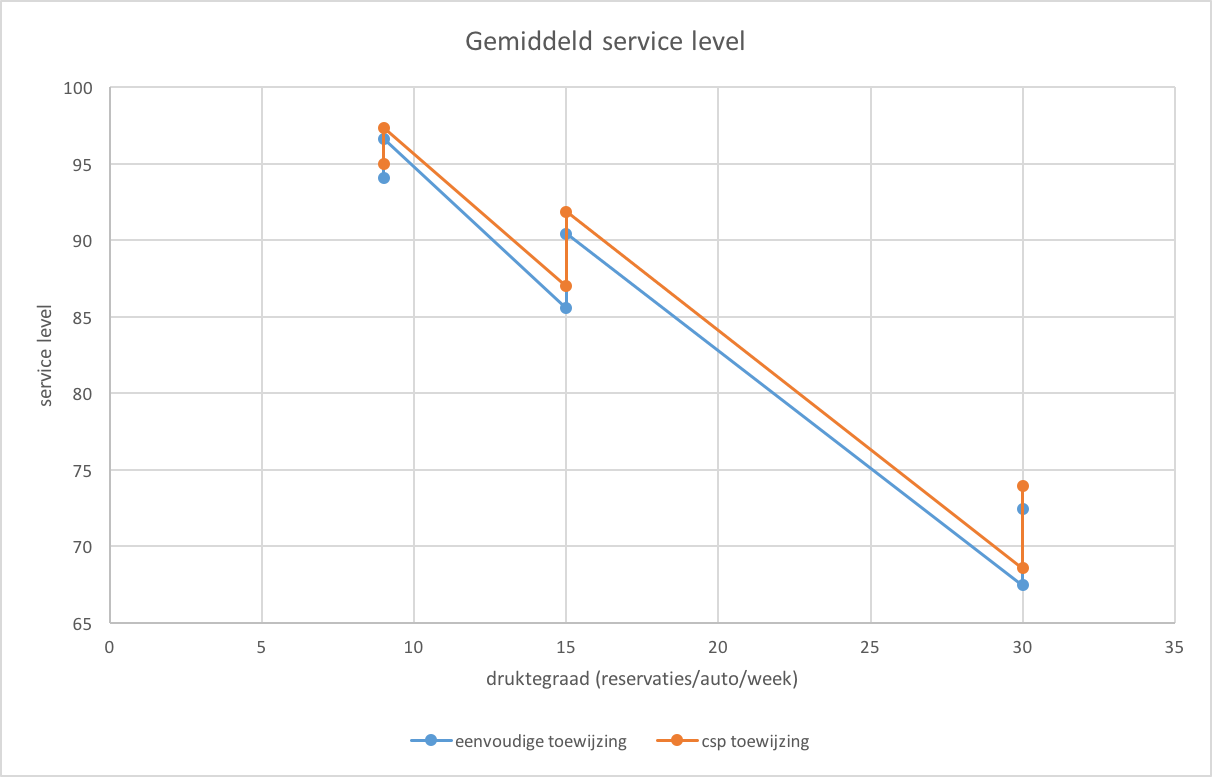
\includegraphics[width=\textwidth]{grafiek-gemiddeld-service-level.png}
	\caption[Gemiddeld service level]{Grafiek van het gemiddelde servicel level per drukte graad}
	\label{grafiek:gemiddeld-service-level}
\end{figure}
Figuur \ref{grafiek:gemiddelde-tijd-actief-per-auto} geeft een spreiding weer voor de gemiddelde tijd actief per auto voor de gesimuleerde druktegraden voor zowel de eenvoudige toewijzing als voor de toewijzing met het csp algoritme.
\begin{figure}[h]
	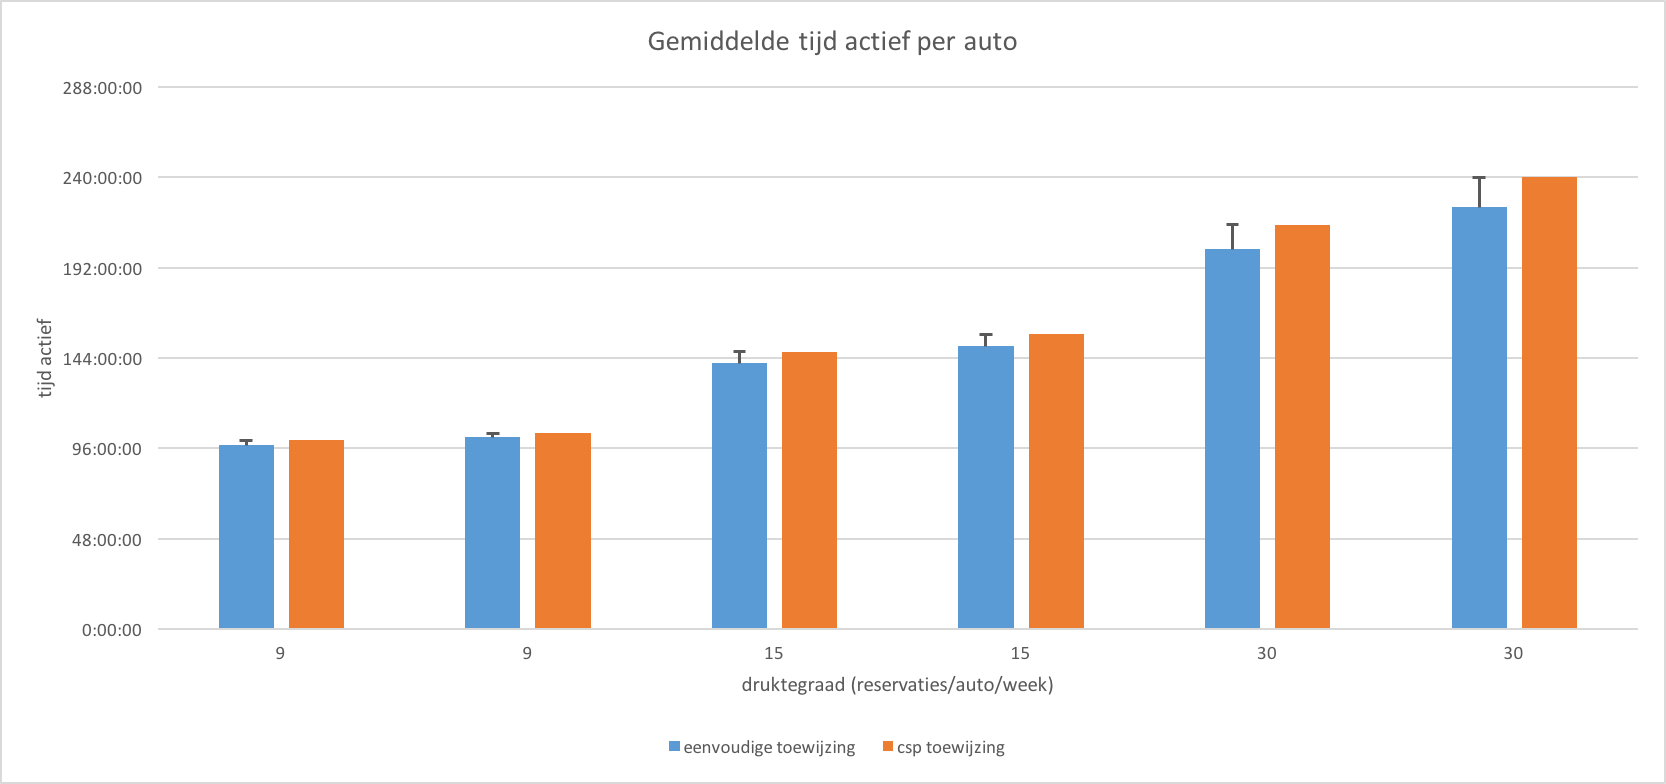
\includegraphics[width=\textwidth]{grafiek-gemiddelde-tijd-actief-per-auto.png}
	\caption[Gemiddelde tijd actief per auto]{Grafiek van de gemiddelde tijd actief per auto per drukte graad}
	\label{grafiek:gemiddelde-tijd-actief-per-auto}
\end{figure}
In figuur \ref{grafiek:gemiddeld-service-level} kan reeds in één oogopslag de meest voor de hand liggende conclusie getrokken worden: het service level voor de toewijzing met het csp algoritme ligt steeds hoger dan de eenvoudige toewijzing. De winstmarges die geboekt worden door het csp algoritme te gebruiken zijn echter klein. Over alle simulaties heen werd er een gemiddelde verhoging van 1,2\% van het service level waargenomen. 
\begin{figure}[h]
	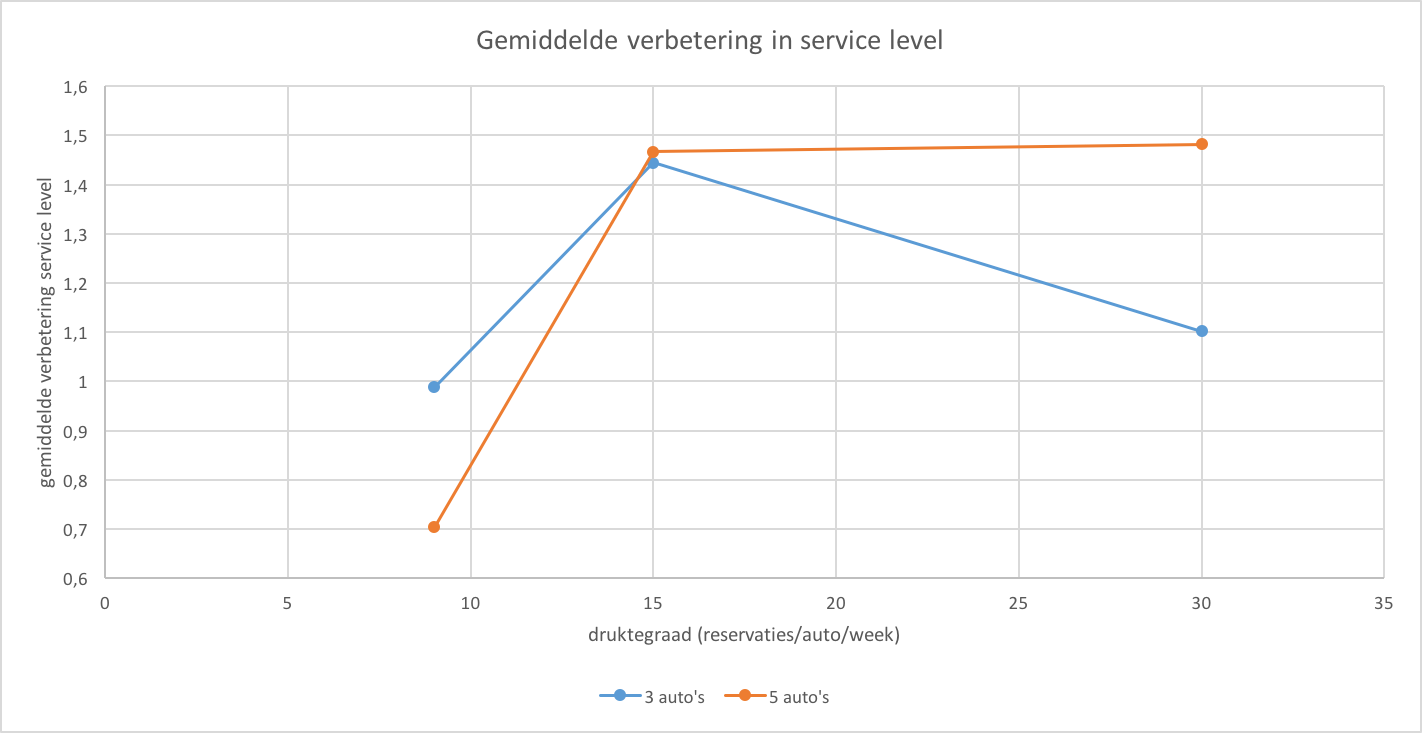
\includegraphics[width=\textwidth]{grafiek-gemiddelde-verbetering-service-level.png}
	\caption[Verbetering service level]{Gemiddelde verbetering van het service level met 3 en 5 auto's}
	\label{grafiek:gemiddelde-verbetering-service-level}
\end{figure}
Uit figuur \ref{grafiek:gemiddelde-verbetering-service-level} blijkt dat de verbeteringen voor hogere druktegraden wel hoger lijken te liggen. Hoe complexer het probleem, met andere woorden, hoe meer auto's en hoe drukker het systeem, hoe groter de mogelijke winstmarges lijken. Deze conclusie kan echter niet met zekerheid getrokken worden. Er zou nog meer getest moeten worden met hogere druktegraden en meer auto's. (zie ook sectie \ref{beperkingen-onderzoek}) De gemeten waarden voor druktegraad 30 met 3 auto's lijkt dit ook tegen te spreken.
Ook de gemiddelde tijd actief per auto ligt voor de csp toewijzing steeds hoger dan voor de eenvoudige toewijzing. Dit wordt weergegeven in figuur \ref{grafiek:gemiddelde-tijd-actief-per-auto} 
Figuur \ref{grafiek:gemiddelde-verbetering-tijd-actief} toont de gemiddelde verbetering van de tijd dat een auto actief was voor 3 en 5 auto's. Deze grafiek ondersteund de conclusie dat hoe complexer het probleem het groter de winstmarge. De rechte die de data voor 5 auto's verbindt stijgt immers steiler dan die voor 3 auto's.
\begin{figure}[h]
	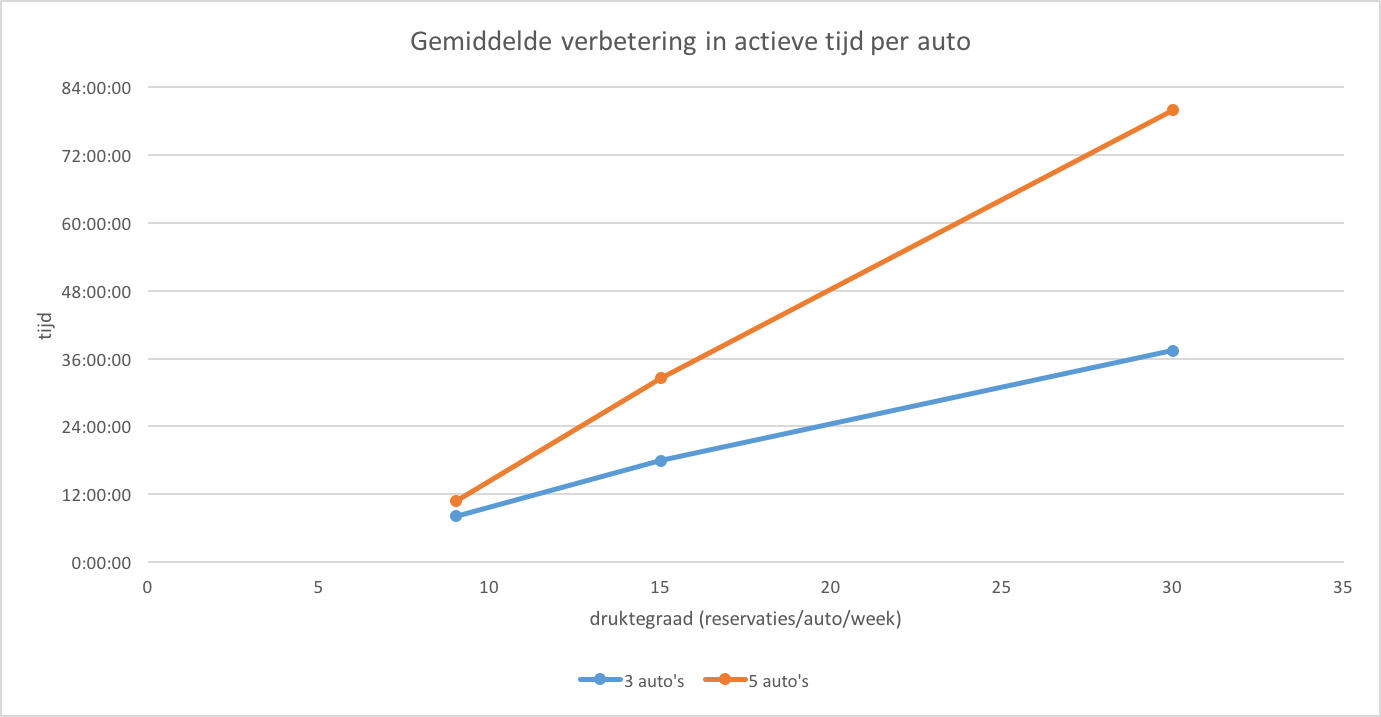
\includegraphics[width=\textwidth]{grafiek-gemiddelde-verbetering-tijd-actief-per-auto.png}
	\caption[Verbetering tijd actief per auto]{Gemiddelde verbetering van de tijd actief per auto voor 3 en 5 auto's}
	\label{grafiek:gemiddelde-verbetering-tijd-actief}
\end{figure}


\section{Antwoord op de onderzoeksvraag}
De onderzoeksvraag die geformuleerd werd in het begin van deze onderzoekstekst luidde als volgt: ``Stijgt het service level en de gebruiksduur van de auto's van Partago  wanneer de gebruikers geen specifieke auto's reserveren, maar enkel een zone?'' Vertaalt naar hoe dit onderzoek gevoerd werd: stijgt het service level en de gebruiksduur van de auto's van Partago met een csp toewijzing ten opzichte van een eenvoudige toewijzing. Als de onderzoeksvraag als een ja-nee vraag geïnterpreteerd wordt dan is het antwoord ``ja''. De winstmarges voor zowel het service level als voor de tijd actief per auto zijn echter relatief klein. In het prijsmodel van Partago is de gereserveerde tijd één van de factoren die de prijs van een rit bepaald. Het is dan ook nuttig om de auto's actiever te maken, ook al is dit maar een beetje. In het huidige prijsmodel is de gemiddelde kostprijs per 3euro/uur voor de gebruiker. Afhankelijk van de druktegraad kan er dus per auto wel meer verdiend worden. Of deze financiële winstmarges opwegen ten opzichte van de kost dat het met zich zou meebrengen om de software van het systeem hieraan aan te passen is een oefening die in dit onderzoek moeilijk gemaakt kan worden, maar met de relatief kleine winstmarge van 1,2\% voor het service level wordt een voorzichtige ``nee'' geformuleerd op deze vraag. Moest uit verder onderzoek blijken dat de winstmarges hoger worden bij een nog drukker systeem kan wordt het in de verre toekomst van Partago misschien wel nuttig. Verder onderzoekzoek zal dit moeten uitwijzen.

\section{Beperkingen van dit onderzoek en een aazet tot verder onderzoek} \label{beperkingen-onderzoek}
De eerst grote beperking is het relatief kleine aantal datapunten die gebruikt zijn in dit onderzoek. De originele opzet met het uitvoeren van simulaties met zelf geschreven code was om een groot aantal datapunten te kunnen genereren voor een meer diverse set van parameters van de simulaties. De console-applicatie gebruikt in dit onderzoek is geschreven in Dart, net zoals de rest van het systeem van Partago. Voor de programmeertaal Dart bestaat er echter slechts 1 bibliotheek voor het oplossen van CSP's. Deze software bibliotheek is een zeer eenvoudige en niet performante implementatie zonder gebruik van de verschillende optimalisatiemogelijkheden zoals heuristieken. Hierdoor liep de rekentijd exponentieel op naarmate het probleem complexer werd. De rekentijd voor de uitgevoerde simulaties in dit onderzoek is nu reeds meer dan 100 uur. Verder onderzoek zou dit onderzoek kunnen herhalen, maar om het CSP op te lossen gebruik maken van meer performante manieren zoals de OptaPlanner gerefereerd in het onderzoeksvoorstel van dit onderzoek. 
Een tweede grote beperking van dit onderzoek is dat voor de toewijzing van een auto aan een reservering er vanuit werd gegaan dat alle reservaties voor de dag gekend zijn voor de start van de eerste reservatie. Op dit tijdstip wordt het CSP probleem opgelost. In de praktijk komen er gedurende de dag echter nog reservaties bij of is er zelfs spontaan gebruik: mensen die een reservatie maken voor 5 minuten later. Momenteel wordt er in het onderzoek geen rekening gehouden met het tijdstip waarop de reservatie gemaakt werd. Deze informatie bevindt zich echter wel in de originele dataset van Partago-reservaties. Verder onderzoek zou wel kunnen gebruik kunnen maken van dit dataveld. Reservaties die dan reeds gestart of gepasseerd op de moment van toekomen van een reservatie mogen dan geen deel meer uitmaken van het CSP probleem.    



%%=============================================================================
%% Bijlagen
%%=============================================================================

\appendix
\renewcommand{\chaptername}{Appendix}

%%---------- Onderzoeksvoorstel -----------------------------------------------

\chapter{Onderzoeksvoorstel}

Het onderwerp van deze bachelorproef is gebaseerd op een onderzoeksvoorstel dat vooraf werd beoordeeld door de promotor. Dat voorstel is opgenomen in deze bijlage.

% Verwijzing naar het bestand met de inhoud van het onderzoeksvoorstel
%---------- Inleiding ---------------------------------------------------------
\section{Introductie} % The \section*{} command stops section numbering
\label{sec:introductie}
Partago is een coöperatie (co-op) met als missie een leefbare omgeving te helpen creëren. Dit doen we door samen elektrisch te rijden. Partago stelt elektrische deelauto's ter beschikking aan zijn leden. Hiervoor heeft Partago een eigen platform ontwikkeld. In 2019 wil Partago als co-op met IT-capaciteit, via een overkoepelende organisatie, het deelplatform ter beschikking stellen aan andere elektrische deelautocoöperaties over heel Europa.

Partago is oorspronkelijk ontstaan in Gent, maar de interesse vanuit andere gemeenten neemt volop toe. Ook in Gent zelf groeit de coöperatie. De vloot in eigen beheer neemt dan ook aan een sneltempo toe. 

Bij het opschalen van een systeem denkt men klassiek eerst aan de niet-functionele vereisten. De groeiende vloot en het groeiend aantal gebruikers botst echter ook op enkele functionele limitaties van het huidige systeem. Het huidige reservatiesysteem dient opgeschaald te worden om met de meer complexe omgang van de coöperatie en die van andere coöperaties te kunnen omgaan. In wat volgt zullen de huidige functionele limitaties geschetst worden. 

%---------- Stand van zaken ---------------------------------------------------

\section{State-of-the-art}
\label{sec:state-of-the-art}
\subsection{Huidig reservatiesysteem}
Vooraleer coöperanten gebruik mogen maken van een deelauto dient deze gereserveerd worden. Auto's staan verspreid over het werkingsgebied. Werkingsgebieden zijn onderverdeeld in verschillende zones of wijken. Een zone is de thuisbasis van een auto. Binnen één zone kunnen evenwel verschillende parkeerplaatsen zijn waar de auto zich bevindt: een publieke laadpaal, een parkeerplaats gereserveerd voor deelauto's, etc. Via de Partago app kunnen er reservaties worden gemaakt voor een specifieke auto. Indien de auto beschikbaar is wordt deze toegewezen aan het account van de gebruiker en kan de gebruiker de auto openen met de app. Tussen twee reservaties wordt een buffertijd voorzien zodat de auto's terug kunnen opladen.   

\subsection{Basisprobleem}
Gebruikers maken een reservatie per auto. Nu Partago groeit geeft dit echter geen optimaal gebruik van auto's wanneer er in één zone meerdere auto's zijn. 
We schetsen het probleem dat zich voordoet aan de hand van een eenvoudig voorbeeld: 

In de stationswijk zijn er 2 Partago deelauto's. Jan maakt een reservatie voor auto1 van 10h-12h. Piet maakt een reservatie voor auto2 van 14h-16h. Ilse, die ook woont in de stationswijk, wil een auto reserveren tussen 11h-15h. Het systeem zal echter melden dat dit niet mogelijk is. Om 11h is auto1 nog in gebruik en om 15h is auto2 al bezet. Moesten echter de reservaties van Jan en Piet beide voor auto1 zijn kon Ilse wel auto2 gebruiken.

Bovenstaand eenvoudig voorbeeld wordt snel heel complex wanneer er meerdere gebruikers, reservatieaanvragen en deelauto's bijkomen in het vraagstuk.
Een planningprobleem behoord tot de NP-complete problemen. Zulke problemen worden snel onhandelbaar en kunnen niet opgelost worden met combinatoriek. Planningproblemen hebben vaak maar toegang tot een beperkt aantal middelen. Als resultaat hiervan zijn er vaak gecompliceerde beperkingen (constraints). \autocite{negnevitsky}
NP-complete problemen wil zeggen dat het eenvoudig is om een een gegeven oplossing te verifiëren, maar dat er geen eenvoudige manier bestaat om een optimale oplossing te vinden. \autocite{manueloptaplanner}

We kunnen het basisprobleem herleiden tot een Constraint Satisfaction Problem (of CSP). Een CSP is gedefinieerd door een set \textbf{variabelen} $X_{1}$, $X_{2},...,X_{n}$ en een set \textbf{constraints} $C_{1}, C_{2},...C_{m}$. Elke variabele $X_{i}$ heeft een niet leeg \textbf{domein} $D_{i}$ van mogelijke waarden. Elke constraint $C_{i}$ heeft betrekking tot een subset van de variabelen en specifieerd de mogelijke combinaties van waarden voor deze subset. Een toestand van het probleem is gedefinieerd als een \textbf{toewijzing} van waarden aan sommige van de variabelen $X_{i} =  v_{i}, X_{j} = v_{j}$... Een toewijzing dat geen enkele van de constraints schendt is een \textbf{consistente} of legale toewijzing. Een volledige toewijzing of \textbf{oplossing} van het CSP is een toewijzing waarin alle variabelen vernoemd worden en aan alle constraints is voldaan. Soms moet een oplossing van een CSP er ook naar streven een strafscore te minimaliseren. \autocite{norvig}

\subsection{Bijkomende complexiteiten}
Het is niet moeilijk om enkele extra beperkingen van het reservatieprobleem te formuleren die de complexiteit enorm doen toenemen. In wat volgt is een beperkte lijst van enkele van de beperkingen. Het vervolledigen van deze lijst van beperkingen zal ook een belangrijk plaats innemen in het onderzoek.
\begin{itemize}
	\item Partago heeft 2 soorten auto's in de aanbieding. Een elektrische stadswagen en een elektrische bestelwagen. Voor sommige cooperanten maakt het misschien niet uit welke auto ze krijgen toegewezen, maar iemand die de ruimte van een bestelwagen nodig heeft moet dit wel nog kunnen aangeven.
	\item Sommige auto's zijn niet altijd beschikbaar tijdens de kantooruren omdat deze gebruikt worden door een bedrijf of een gemeenten. Met het huidige reservatiesysteem worden deze auto's weinig gekozen. Een optimalisatie van de reserveringen is extra interessant voor deze wagens.
	\item Batterijstatus van de wagen moet in overeenstemming zijn met de geplande rit. Er zijn ook wagen van het zelfde type met een grotere batterij. Voor een langere rit is het gebruik van een wagen met grotere autonomie dus aangewezen.
	\item In de huidige zone is er misschien geen auto beschikbaar, maar in een naburige zone op wandelafstand misschien wel. Ook met deze auto's zou rekening gehouden moeten worden.
	\item Ook een auto die stilstaat heeft een waarde. Enerzijds marketing, maar anderzijds verhoogt dit ook het gevoel van beschikbaarheid. 
	\item Een specifieke auto moet voor een specifieke periode op onbeschikbaar kunnen worden geplaatst bijvoorbeeld voor onderhoud.
\end{itemize}

In het reservatieprobleem kunnen er twee soorten constraints onderscheden worden: \textbf{harde constraints}, deze moeten kost wat kost voldaan worden anders hebben we geen aanvaardbare toewijzing voor de onderneming en \textbf{zachte constraints}, constraints waaraan zoveel mogelijk voldaan dient te worden. Indien er niet aan één van deze zachte constraints voldaan kan worden krijgt onze oplossing een gewogen strafscore $w_{m} \geq 0$. Hiernaast definiëren we de variabele $k_{m} \geq 0$ als het aantal keer dat de m-de constraint gebroken is. Tijdens het oplossen van het probleem dient dus de functie $\rho(\,s)\,=\sum\limits_{m} w_{m}k_{m}$ geminimaliseerd worden. \autocite{santos}   


% Voor literatuurverwijzingen zijn er twee belangrijke commando's:
% \autocite{KEY} => (Auteur, jaartal) Gebruik dit als de naam van de auteur
%   geen onderdeel is van de zin.
% \textcite{KEY} => Auteur (jaartal)  Gebruik dit als de auteursnaam wel een
%   functie heeft in de zin (bv. ``Uit onderzoek door Doll & Hill (1954) bleek
%   ...'')

%---------- Methodologie ------------------------------------------------------
\section{Methodologie}
\label{sec:methodologie}
Een CSP oplossen is een complexe aangelegenheid. Voor het oplossen van deze complexe problemen bestaan er softwarebibliotheken. Een eerste deel van het onderzoek zal zijn om te onderzoeken of het CSP-probleem opgelost kan worden binnen de huidige technologiestack en indien niet welke externe softwarebibliotheek de meest logische keuze lijkt om het oplossen eenvoudiger te maken. Eens het CSP opgelost kan worden zal er onderzocht worden hoe dit geïntegreerd kan worden in de huidige architectuur van het systeem. 

Het doel van het onderzoek is niet het oplijsten van de verschillende manieren om het vraagstuk op te lossen. Er zijn tientallen verschillende softwarepakketten en nog eens meer algoritmen om CSP problemen mee op te lossen. Deze allemaal vergelijken zou een onderzoek op zich zijn. Het doel van dit onderzoek is om \textit{een} manier te identificeren en te onderzoeken hoe deze geïntegreerd kan worden in de huidige architectuur en de mogelijke implicaties hiervan te identificeren. De eindscriptie zal als leiddraad dienen voor de ontwikkelaars van Partago om een meer geoptimaliseerd reservatiesysteem te ontwikkelen. 

Het onderzoek zal uit drie stappen bestaan:
\begin{enumerate}
	\item Welke software/algoritme voor het oplossen van het CSP 
	\item De gekozen software integreren in huidige architectuur van het systeem met mogelijkheid van migratie
	\item Implicaties identificeren voor de user interface en de user experience.
\end{enumerate}

%---------- Verwachte resultaten ----------------------------------------------
\section{Verwachte resultaten}
\label{sec:verwachte_resultaten}
Voor het oplossen van het CSP is de meest voor de handliggende manier het gebruik van de softwarebibliotheek Optaplanner. Zelf een algoritme implementeren binnen de huidige technologiestack lijkt buiten de kennis, mogelijkheden en tijdsbestek te liggen van het ontwikkelaarsteam.
Optaplanner is de meest aantoongevende CSP oplosser. Het is een lichtgewicht en integreerbare planning engine. Het stelt normale Java programmeurs in staat om optimalisatieproblemen efficient op te lossen. \autocite{optaplanner} Het huidige reservatiesysteem maakt grotendeels gebruik van Google technologieën. Een alternatief dat het te bekijken waard is zijn de OR-tools door Google. \autocite{ortools} Echter de meeste vakliteratuur nu reeds geraadpleegd vermeld Optaplanner. Een meer uitgebreide studie dient uitsluitsel te geven over welke software gebruikt gaat worden waarbij de werkbaarheid voor de ontwikkelaars van Partago de doorslaggevende factor zal zijn. De gekozen softwarebibliotheek zal specifiek geimplementeerd en geconfigureerd moeten worden zodat het het reservatieprobleem kan oplossen. Dit ligt ook binnen het bestek van dit onderzoek. Een demo-run met dummydata van auto's, zones en cooperanten dient bewijs te leveren dat de gekozen softwarebibliotheek in staat is om het probleem op een tijdsperformante manier op te lossen. 

Door de gebrekkige ervaring hoe het huidige reservatiesysteem op architecturaal niveau is opgebouwd is het niet mogelijk om grote architectuurwijzigingen nu reeds te identificeren. Optaplanner kan met behulp frameworks Camel of RESTEasy beschikbaar worden gesteld als REST service. \autocite{manualoptaplanner} In een microservice architectuur lijkt dit een mooie oplossing om een geavanceerder reservatiesysteem te integreren met de rest van de gebruikte technologiestack.

Het huidige reservatieproces voor een gebruiker is heel eenvoudig. Er wordt gereserveerd voor een bepaalde periode voor een bepaalde auto. Wanneer reservaties niet langer voor een specifieke auto zullen zijn moet de gebruiker wel verschillende van de constraints kunnen bepalen. Er moet bewaakt worden dat dit op een gebruiksvriendelijke manier in de userinterface geïmplementeerd wordt zodat de positieve gebruikerservaring bewaard kan worden.

%Hier beschrijf je welke resultaten je verwacht. Als je metingen en simulaties uitvoert, kan je hier al mock-ups maken van de grafieken samen met de verwachte conclusies. Benoem zeker al je assen en de stukken van de grafiek die je gaat gebruiken. Dit zorgt ervoor dat je concreet weet hoe je je data gaat moeten structureren.%

%---------- Verwachte conclusies ----------------------------------------------
\section{Verwachte conclusies}
\label{sec:verwachte_conclusies}
Als Partago meer en meer coöperanten ten dienste wil zijn is het opschalen van het reservatiesysteem een kritische stap. De beoogde bachelorproef wil het plan uittekenen om deze kritische stap op een doordachte manier te nemen.  


\chapter{Code simulatietool}
De volledige code kan op aanvraag geraadpleegd worden op: https://github.com/timalenus/partago-bp
De code is afhankelijk van gesloten software waarvan Partag cvba eigenaar is. Voor deze reden wordt de volledige broncode niet publiekelijk opgenomen bij deze bachelorproef. Een deel van de code werd wel opgenomen verder in deze appendix.
\lstinputlisting[breaklines=true]{source-code-simulation-tool.dart}

%%---------- Andere bijlagen --------------------------------------------------
% TODO: Voeg hier eventuele andere bijlagen toe
%\input{...}

%%---------- Referentielijst --------------------------------------------------

\printbibliography[heading=bibintoc]

\end{document}
